\title{Chapter 4, Section 2. Exercises 1, 2, and 4 through 9}
\author{
	MTH 594, Prof. Mikael Vejdemo-Johansson \\
	Differential Geometry Independent Study \\
	\\
	Matthew Connelly \\
}
\date{\today}



\documentclass[12pt]{article}

\usepackage[top=.5in, bottom=.75in, left=1in, right=1in]{geometry}
\usepackage{amssymb}
\usepackage{amsmath}
\usepackage{graphicx}
\usepackage{subcaption}


\begin{document}
\maketitle

\section*{Exercise 4.2.1}
Show that, if $f(x, y)$ is a smooth function, its graph
$$
\lbrace(x,y,z) \in \mathbb{R}^3 \ | \ z = f(x,y) \rbrace
$$
is a smooth surface with atlas consisting of the single regular surface patch
$$
\sigma (u,v) = (u,v,f(u,v)).
$$
In fact, every surface is "locally" of this type - see Exercise 5.6.4.

\vspace{1cm}
\hrule
\vspace{1cm}

If $f(x,y)$ is smooth, that implies $f \in C^n$; $f$ is continuously differentiable to the $n$th order.\\
If $z = f(x,y)$ is a smooth surface, then $z \in C^n$, as well.\\
\indent
To show that $z$ is a surface, let there be open sets $U$ and $W$ in $\mathbb{R}^2$ and $\mathbb{R}^3$, respectively.\\
\begin{figure}[h!]
  \centering
      \begin{subfigure}[b]{0.5\linewidth}
    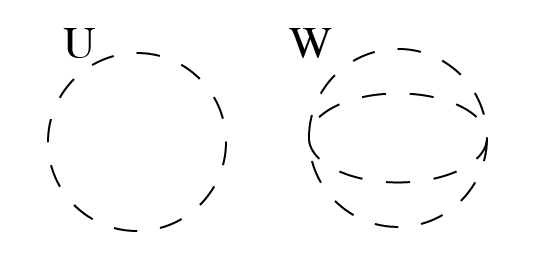
\includegraphics[width=\linewidth]{./assets/4-2-1/u-and-w.png}
  \end{subfigure}
  \end{figure}
  \\
  \clearpage
Then, let there be some mapping function $F$, that will map $U$ to the intersection of $z$ and $W$:\\
$$
F: U \rightarrow z \cap W
$$
$$
F^{-1}: z \cap W \rightarrow U
$$
Which could be loosely visualized as the following if doing so proves useful:\\
\begin{figure}[h!]
  \centering
      \begin{subfigure}[b]{0.5\linewidth}
    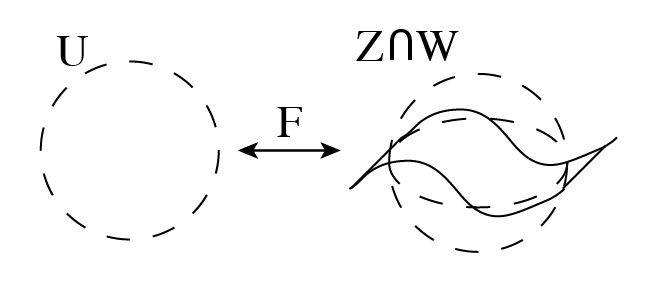
\includegraphics[width=\linewidth]{./assets/4-2-1/u-and-w-mapping.png}
  \end{subfigure}
  \end{figure}
  \\
\indent
Meaning, $F$ is a smooth, bijective map, and therefore a homeomorphism between $z \cap W$ and $U$.\\
\indent
$z$ is now a surface because it can be made into surface patches (homeomorphic open subsets).\\

\noindent
\underline{$z$ has a single regular surface patch:}\\\\
As stated in the problem, let $z$'s surface patch be parametrized as the following:
$$
\sigma (u,v) = (u,v,f(u,v)).
$$
Then we can take for granted that $(u,v) \in U$ and $U \in \mathbb{R}^2$.\\
\indent
We can also use the aforementioned mapping function $F$ to map $(u,v) \in U$ to $z \cap W$, but refer to it as $\sigma$ (as it is referred to in the text).\\
\clearpage
Here will follow some information about $z$ that points to its atlas having only a single patch:\\\\
\indent
\emph{Smoothness:}\\
\indent
Because $z$ is smooth (and smooth all over), there are no "holes" or other singularities for all $u$ and $v$ mapped to $z \cap W$ by $\sigma$.\\

\emph{No disjoint points:}\\
\indent
Because $z \cap W$ and $U$ are open, there are no disjoint points within either:
$$
\lbrace u,v \in U \ | \ ||v-u|| < r \rbrace
$$
\indent
Here, $r$ is the radius of $U$ as an open disc. Similarly, $r$ may be the radius of $z \cap W$ as an open ball.\\

$\therefore$, we will be able to approach $r$ in $z \cap W$ from any point and cover the entirety of the surface, showing that $z$'s atlas consists solely of $\sigma$.
\begin{figure}[h!]
  \centering
      \begin{subfigure}[b]{0.5\linewidth}
    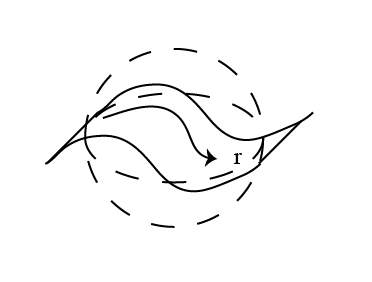
\includegraphics[width=\linewidth]{./assets/4-2-1/approaching-r.png}
  \end{subfigure}
  \end{figure}
  \\
\end{document}
This is never printed
